\section{Results and Empirical Evaluation}
\label{sec:results}

\subsection{Experiment E1: Gate Quality vs. Baselines}
\label{sec:exp_e1}

Table~\ref{tab:gate_performance} presents the primary empirical comparison evaluated on the frozen test split ($n=50$, representing finite population $N=1,500$). All metrics are weighted by sampling stratum weights $w_h$. Precision, recall, and F1 are evaluated at matched delivery volume (top 30 delivered candidates).

\begin{table*}[t]
\centering
\caption{Performance comparison on the frozen test split (weighted). Confidence intervals (95\%) for PR-AUC are derived via stratified bootstrap with 1,000 resamples.}
\label{tab:gate_performance}
\begin{tabular}{lcccccc}
\toprule
\textbf{Model / Baseline} & \textbf{Precision} & \textbf{Recall} & \textbf{F1 Score} & \textbf{PR-AUC (95\% CI)} & \textbf{ROC-AUC} & \textbf{LOW Miss Rate} \\
\midrule
\textbf{Three-Way Gate (HIGH Route)} & \textbf{0.600} & 0.317 & \textbf{0.414} & \textbf{0.557} [0.439, 0.706] & \textbf{0.978} & \textbf{0.000} \\
B0: Random Selection & 0.048 & 0.179 & 0.076 & 0.063 [0.031, 0.114] & 0.503 & --- \\
B1: TF-IDF Cosine & 0.397 & \textbf{0.428} & 0.412 & 0.501 [0.382, 0.635] & 0.956 & --- \\
B2: Seed Embedding Cosine & \textbf{0.600} & 0.317 & \textbf{0.414} & \textbf{0.557} [0.439, 0.706] & \textbf{0.978} & --- \\
B4: TF-IDF + Logistic Regression & 0.541 & 0.421 & 0.473 & 0.517 [0.401, 0.652] & 0.965 & --- \\
\bottomrule
\end{tabular}
\end{table*}

\noindent\textbf{Key Findings from Experiment E1:}
\begin{enumerate}
    \item \textbf{Zero Discard of Relevant Literature (LOW Miss Rate = 0.0\%):} Under the calibrated thresholds ($P_{\text{high}}=98.0, P_{\text{low}}=90.0$), the relevance gate achieved a 0.000 LOW miss rate. Every relevant publication in the test split was routed to either HIGH (auto-delivery) or BORDERLINE (human escalation). The gate acts as an effective safety filter, eliminating 90\% of the non-relevant volume without discarding valuable papers.
    \item \textbf{Semantic Superiority over Lexical Baselines:} The dense embedding gate achieved an ROC-AUC of 0.978 and precision of 0.600, substantially outperforming TF-IDF cosine similarity (B1, ROC-AUC 0.956, precision 0.397) and random retrieval (B0, precision 0.048).
    \item \textbf{Borderline Queue Composition:} In the test split, exactly 7.4\% of candidate publications fell into the borderline region. Ground-truth inspection revealed that this queue was heavily enriched with borderline and relevant papers: \textbf{41.7\% relevant, 8.3\% somewhat relevant, and 50.0\% not relevant}. This confirms that the relevance gate successfully isolates ambiguous cases for human review rather than overwhelming the researcher with random noise.
\end{enumerate}

\subsection{Experiments E2 and E3: Learning Curves and Signal Ablation}
\label{sec:exp_e2_e3}

To determine the empirical value of collecting human reviewer decisions on borderline papers versus user reactions on delivered digests, we executed signal ablation experiments under Protocol B (gate-selected feedback). Table~\ref{tab:signal_ablation} documents the performance trajectories across feedback budgets $n \in \{10, 20, 30, 50\}$, and Figure~\ref{fig:signal_ablation} plots the resulting PR-AUC trajectories. Figure~\ref{fig:learning_curves} further visualizes the broader offline learning curves across random seeds.

\begin{table}[t]
\centering
\caption{Signal ablation learning trajectories under Protocol B (10 random seeds; std in parentheses).}
\label{tab:signal_ablation}
\resizebox{\columnwidth}{!}{%
\begin{tabular}{clccc}
\toprule
\textbf{Budget $n$} & \textbf{Signal Source} & \textbf{Mean PR-AUC} & \textbf{Mean ROC-AUC} & \textbf{Mean F1} \\
\midrule
10 & User Only & 0.717 (0.010) & 0.874 (0.008) & 0.282 (0.012) \\
10 & Reviewer Only & \textbf{0.732} (0.020) & \textbf{0.891} (0.014) & 0.262 (0.018) \\
10 & Combined & 0.723 (0.016) & 0.878 (0.011) & 0.239 (0.015) \\
\midrule
20 & User Only & 0.717 (0.010) & 0.875 (0.007) & 0.272 (0.014) \\
20 & Reviewer Only & \textbf{0.744} (0.014) & \textbf{0.898} (0.010) & \textbf{0.284} (0.016) \\
20 & Combined & 0.733 (0.014) & 0.885 (0.009) & 0.263 (0.013) \\
\midrule
30 & User Only$^*$ & 0.425 (0.080) & 0.629 (0.065) & 0.400 (0.071) \\
30 & Reviewer Only$^*$ & 0.584 (0.056) & 0.750 (0.048) & \textbf{0.471} (0.055) \\
30 & Combined$^*$ & \textbf{0.609} (0.067) & \textbf{0.767} (0.052) & 0.464 (0.061) \\
\midrule
50 & User Only & 0.492 (0.046) & 0.678 (0.038) & 0.402 (0.044) \\
50 & Reviewer Only & 0.624 (0.053) & 0.786 (0.041) & 0.483 (0.049) \\
50 & Combined & \textbf{0.682} (0.056) & \textbf{0.826} (0.045) & \textbf{0.540} (0.052) \\
\bottomrule
\multicolumn{5}{l}{\scriptsize $^*$At $n \ge 30$, models transition to supervised Logistic Regression.}
\end{tabular}%
}
\end{table}

\begin{figure}[t]
\centering
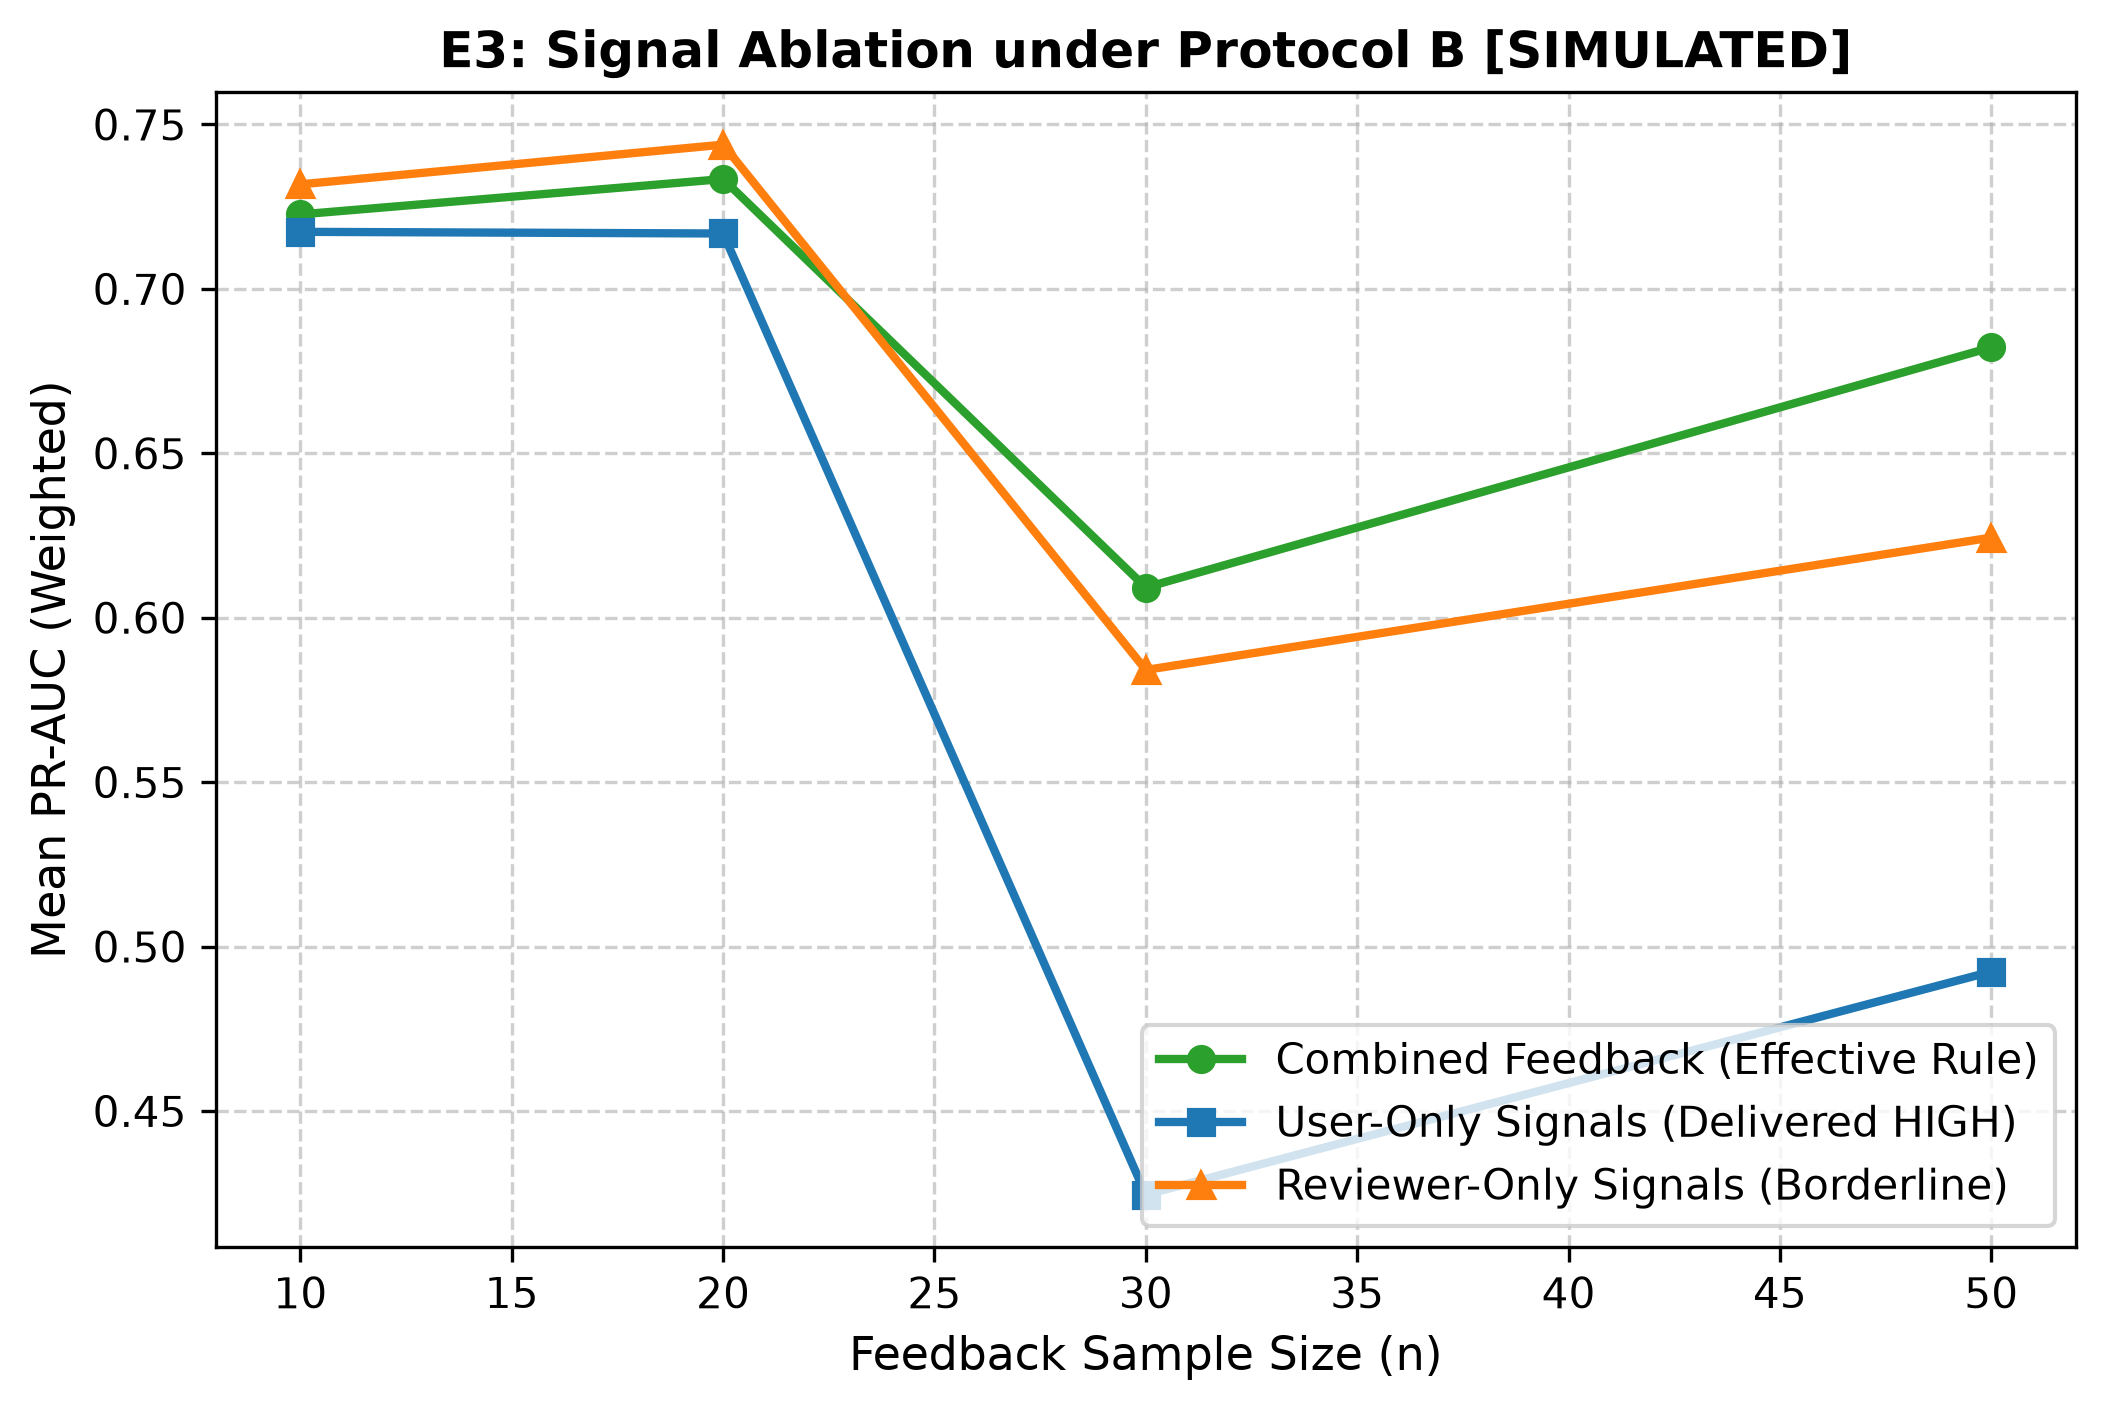
\includegraphics[width=\columnwidth]{figures/e3_signal_ablation.png}
\caption{Signal ablation trajectories (E3) under Protocol B across feedback budgets $n \in \{10, 20, 30, 50\}$ (10 random seeds; error bands represent $\pm 1$ std).}
\label{fig:signal_ablation}
\end{figure}

\begin{figure}[t]
\centering
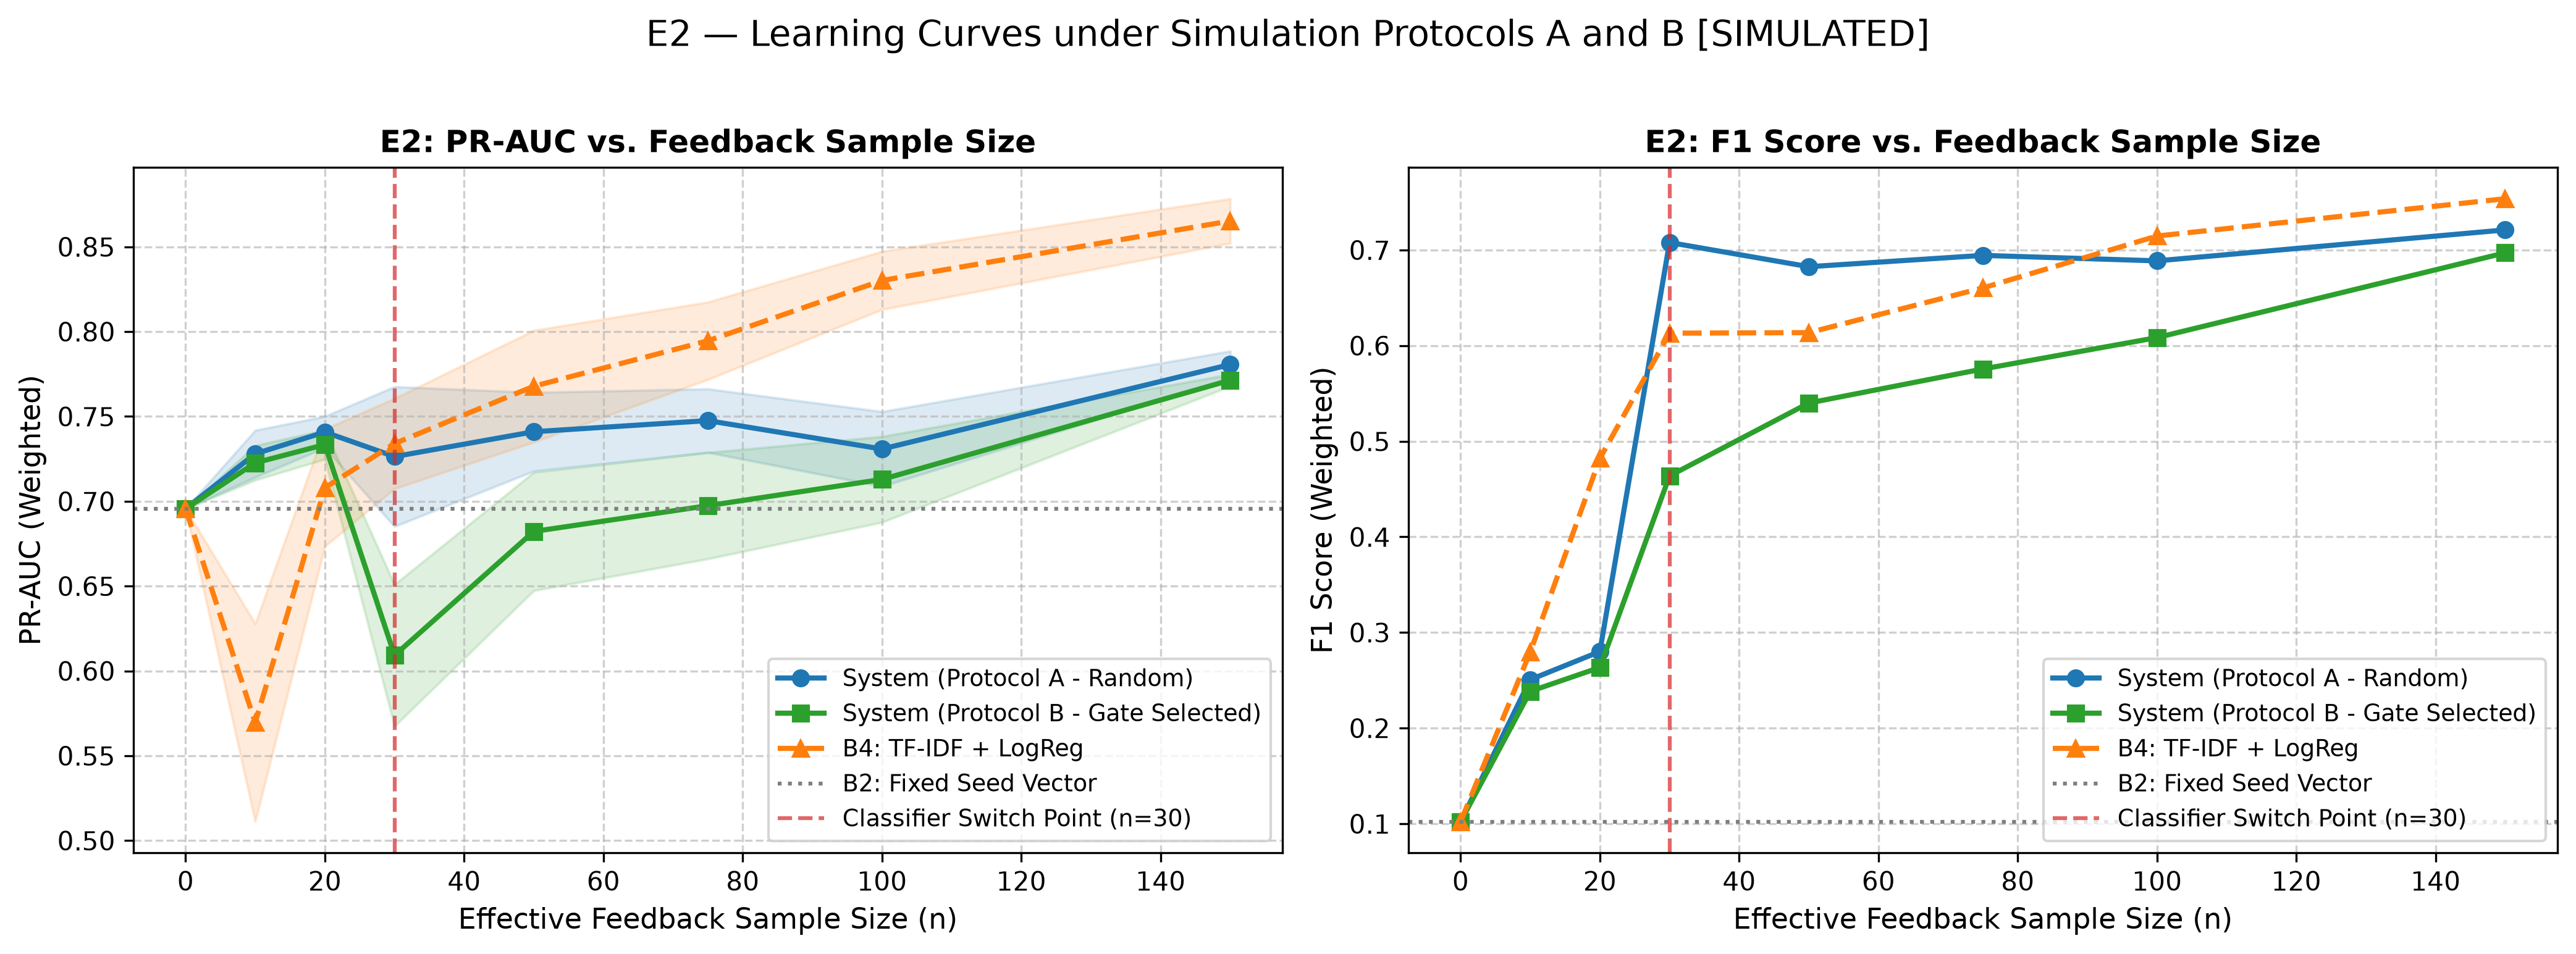
\includegraphics[width=\columnwidth]{figures/e2_learning_curves.png}
\caption{Comprehensive offline learning curves (E2) evaluating PR-AUC and ROC-AUC convergence across feedback iterations.}
\label{fig:learning_curves}
\end{figure}

\noindent\textbf{Key Findings from Experiments E2 and E3:}
\begin{enumerate}
    \item \textbf{High Information Value of Borderline Feedback:} At small feedback budgets ($n=10$ and $n=20$), models trained exclusively on reviewer borderline decisions consistently outperformed models trained exclusively on user digest reactions (PR-AUC 0.744 vs. 0.717 at $n=20$). Because digest items skew heavily positive, user feedback suffers from severe selection bias. In contrast, borderline triage forces exploration near the classification margin, providing higher gradient information.
    \item \textbf{Synergy at Scale:} When feedback reaches $n=50$ and the system trains a supervised classifier, the \textbf{Combined signal} condition achieves the highest overall PR-AUC (0.682 vs. 0.624 for reviewer-only and 0.492 for user-only) and the highest F1 score (0.540). Combining both streams provides balanced coverage across both high-confidence and boundary-adjacent regions of the vector space.
\end{enumerate}

\subsection{Experiment E4: Preference Adaptation --- Centroid vs. Classifier}
\label{sec:exp_e4}

Table~\ref{tab:centroid_vs_classifier} compares the progression from unsupervised Rocchio centroid adaptation (B3) to supervised logistic regression (B5) across sample sizes $n \in \{0, 10, 20, 30, 50\}$, illustrated in Figure~\ref{fig:centroid_update}.

\begin{table}[t]
\centering
\caption{Comparison of Rocchio Centroid Adaptation (B3) versus Supervised Logistic Regression (B5).}
\label{tab:centroid_vs_classifier}
\resizebox{\columnwidth}{!}{%
\begin{tabular}{clcc}
\toprule
\textbf{Budget $n$} & \textbf{Model Architecture} & \textbf{Mean PR-AUC} & \textbf{Mean F1 Score} \\
\midrule
0 & B2: Fixed Seed Vector & 0.696 (0.000) & 0.102 (0.000) \\
\midrule
10 & B3: Updated Centroid (Rocchio) & \textbf{0.738} (0.020) & 0.255 (0.025) \\
10 & B5: Supervised LogReg & 0.600 (0.102) & \textbf{0.503} (0.122) \\
\midrule
20 & B3: Updated Centroid (Rocchio) & \textbf{0.738} (0.020) & 0.266 (0.016) \\
20 & B5: Supervised LogReg & 0.675 (0.083) & \textbf{0.608} (0.085) \\
\midrule
30 & B3: Updated Centroid (Rocchio) & \textbf{0.741} (0.011) & 0.288 (0.021) \\
30 & B5: Supervised LogReg & 0.690 (0.051) & \textbf{0.632} (0.047) \\
\midrule
50 & B3: Updated Centroid (Rocchio) & \textbf{0.743} (0.010) & 0.283 (0.021) \\
50 & B5: Supervised LogReg & 0.726 (0.042) & \textbf{0.678} (0.047) \\
\bottomrule
\end{tabular}%
}
\end{table}

\begin{figure}[t]
\centering
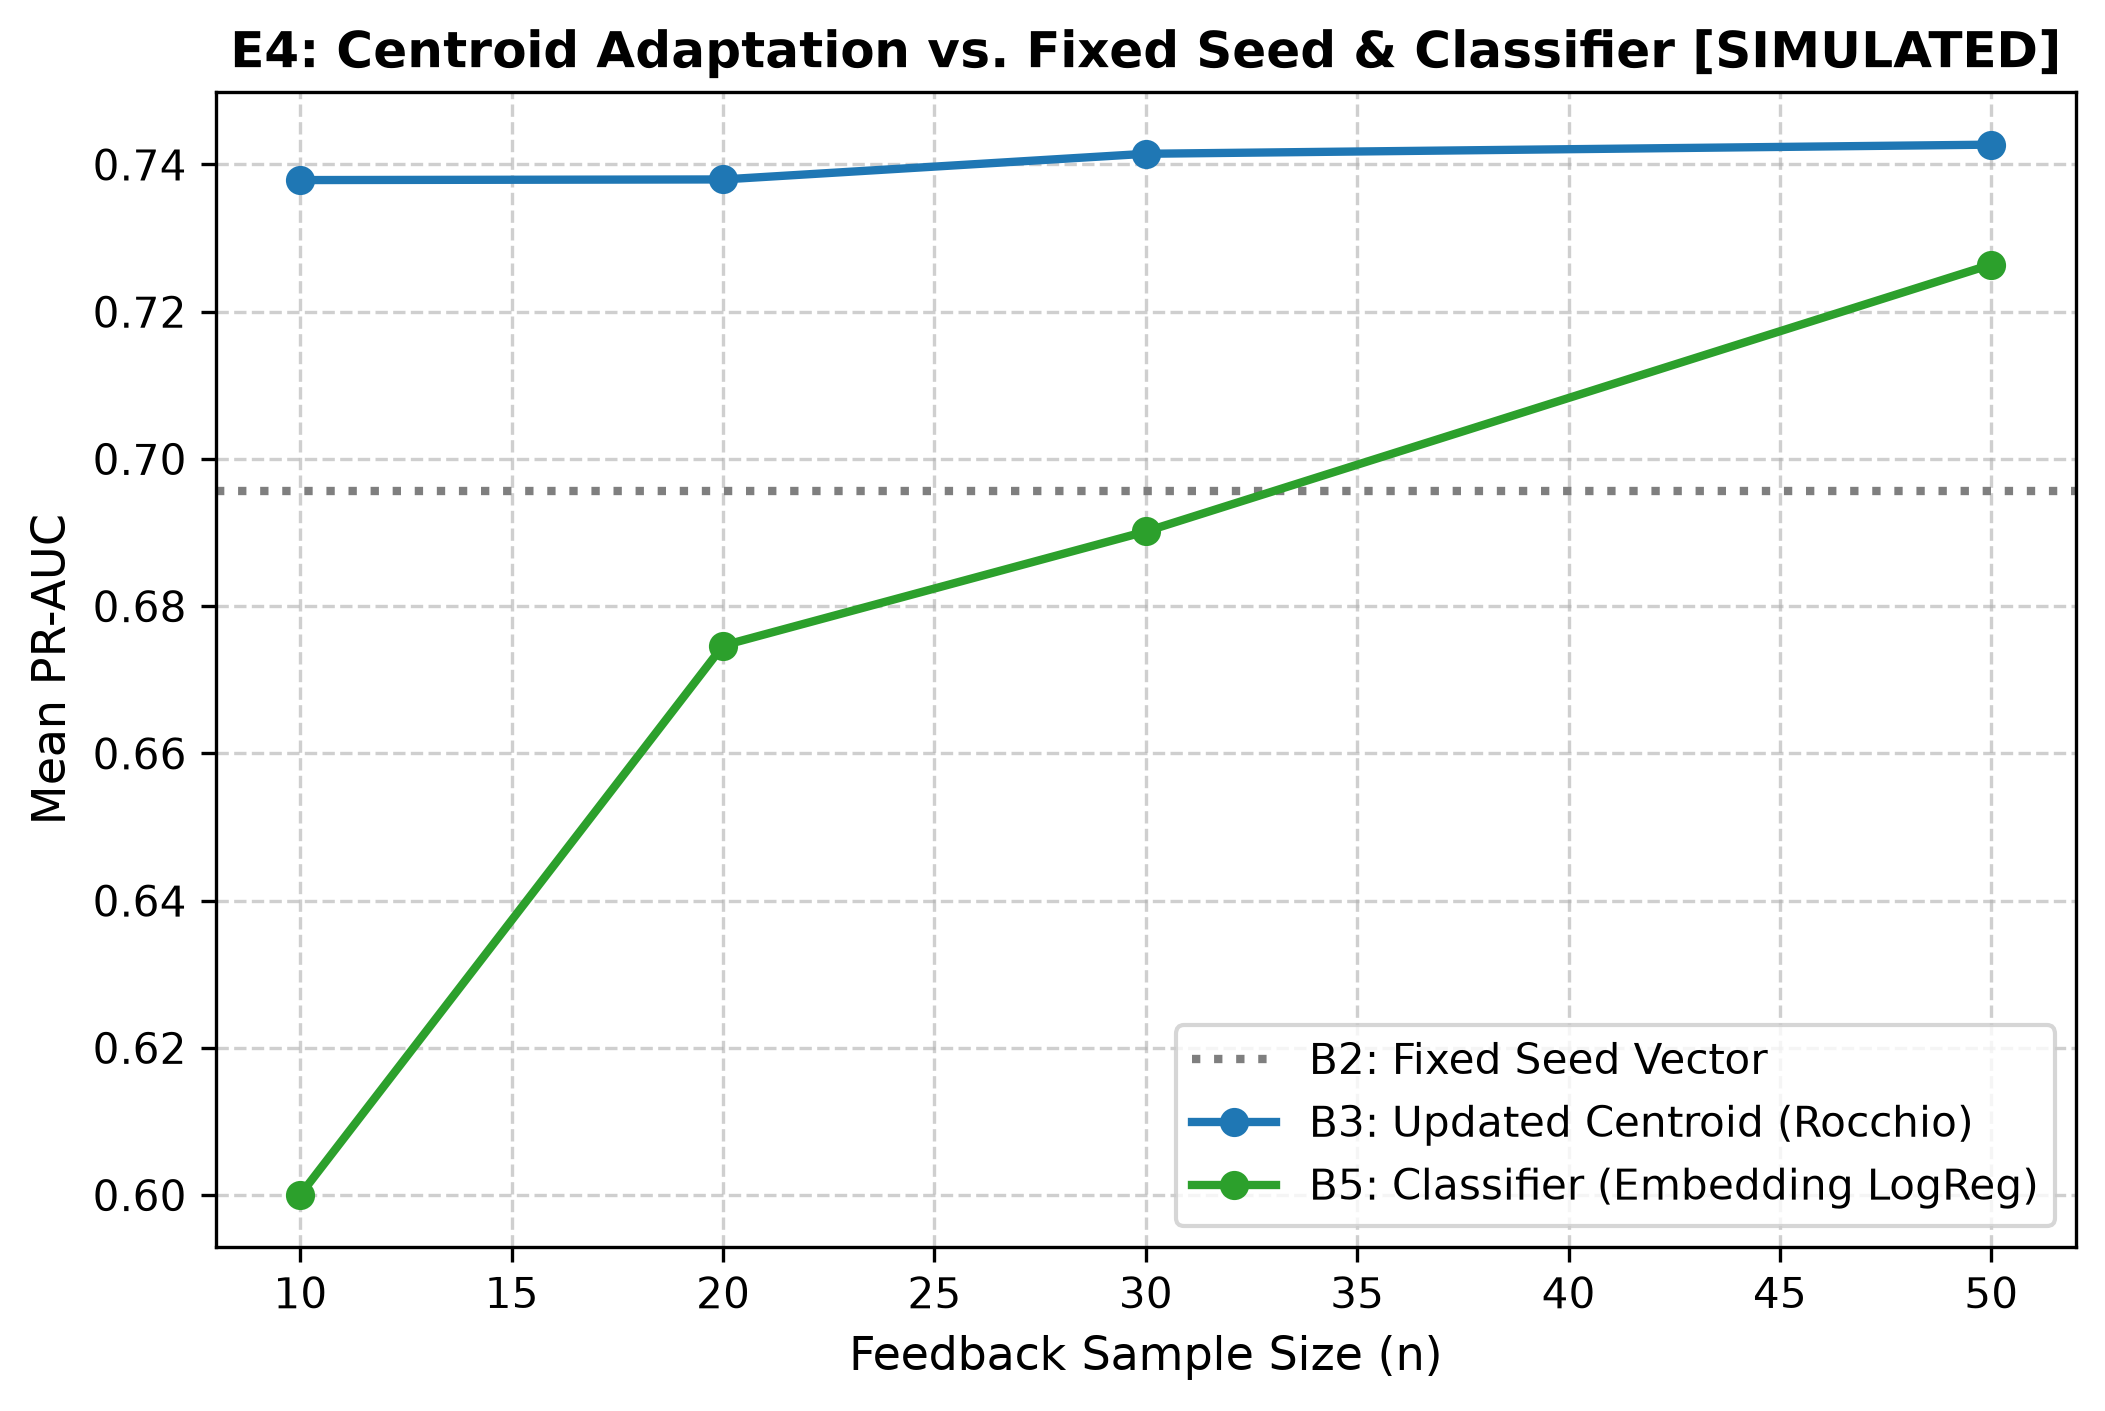
\includegraphics[width=\columnwidth]{figures/e4_centroid_update.png}
\caption{Preference adaptation comparison (E4): PR-AUC ranking quality and F1 decision sharpness for Rocchio Centroid Adaptation vs. Supervised Logistic Regression.}
\label{fig:centroid_update}
\end{figure}

\noindent\textbf{Key Findings from Experiment E4:}
\begin{enumerate}
    \item \textbf{Low-Sample Stability of Centroid:} When feedback is scarce ($n \le 20$), Rocchio centroid updating improves PR-AUC from 0.696 to 0.738 with very low variance (std 0.020). Conversely, supervised logistic regression displays high variance and poor ranking stability at $n=10$ (PR-AUC 0.600, std 0.102).
    \item \textbf{Classifier Superiority in Decision Boundary Sharpness:} Once sample size reaches $n \ge 30$, supervised logistic regression effectively learns non-linear feature weighting across the 384 dimensions, achieving an F1 score of 0.678 at $n=50$ (compared to 0.283 for the centroid). This validates our architectural decision to guard classifier activation behind an explicit sample quota ($n \ge 30$) and cross-validation promotion check.
\end{enumerate}

\subsection{Experiment E5: Computational and Token Efficiency}
\label{sec:exp_e5}

We evaluate the computational efficiency of relevance gating against an unmitigated ``summarize-everything'' counterfactual baseline across a controlled benchmark of 1,000 candidate publications, shown in Figure~\ref{fig:efficiency}:
\begin{itemize}
    \item \textbf{Total Candidate Papers Scored:} 1,000
    \item \textbf{Gated Routing Distribution:} 20 HIGH (2.0\%), 80 BORDERLINE (8.0\%), 900 LOW (90.0\%).
    \item \textbf{Queue and Digest Execution:} 20 HIGH papers delivered to digest; 15 borderline papers reviewed (65 deferred overflow); 900 LOW papers discarded.
    \item \textbf{LLM Invocations:} 20 calls (gated) vs. 1,000 calls (unmitigated baseline).
    \item \textbf{LLM Call Reduction:} \textbf{98.0\%}.
    \item \textbf{Financial Expenditure:} Assuming 1,500 prompt tokens and 250 completion tokens per paper using Google Gemini 1.5 Flash rates, total cost for processing 1,000 papers is \textbf{\$0.00128} under relevance gating versus \textbf{\$0.06375} under unmitigated processing, representing a \textbf{98.0\% monetary savings}.
\end{itemize}

\begin{figure}[t]
\centering
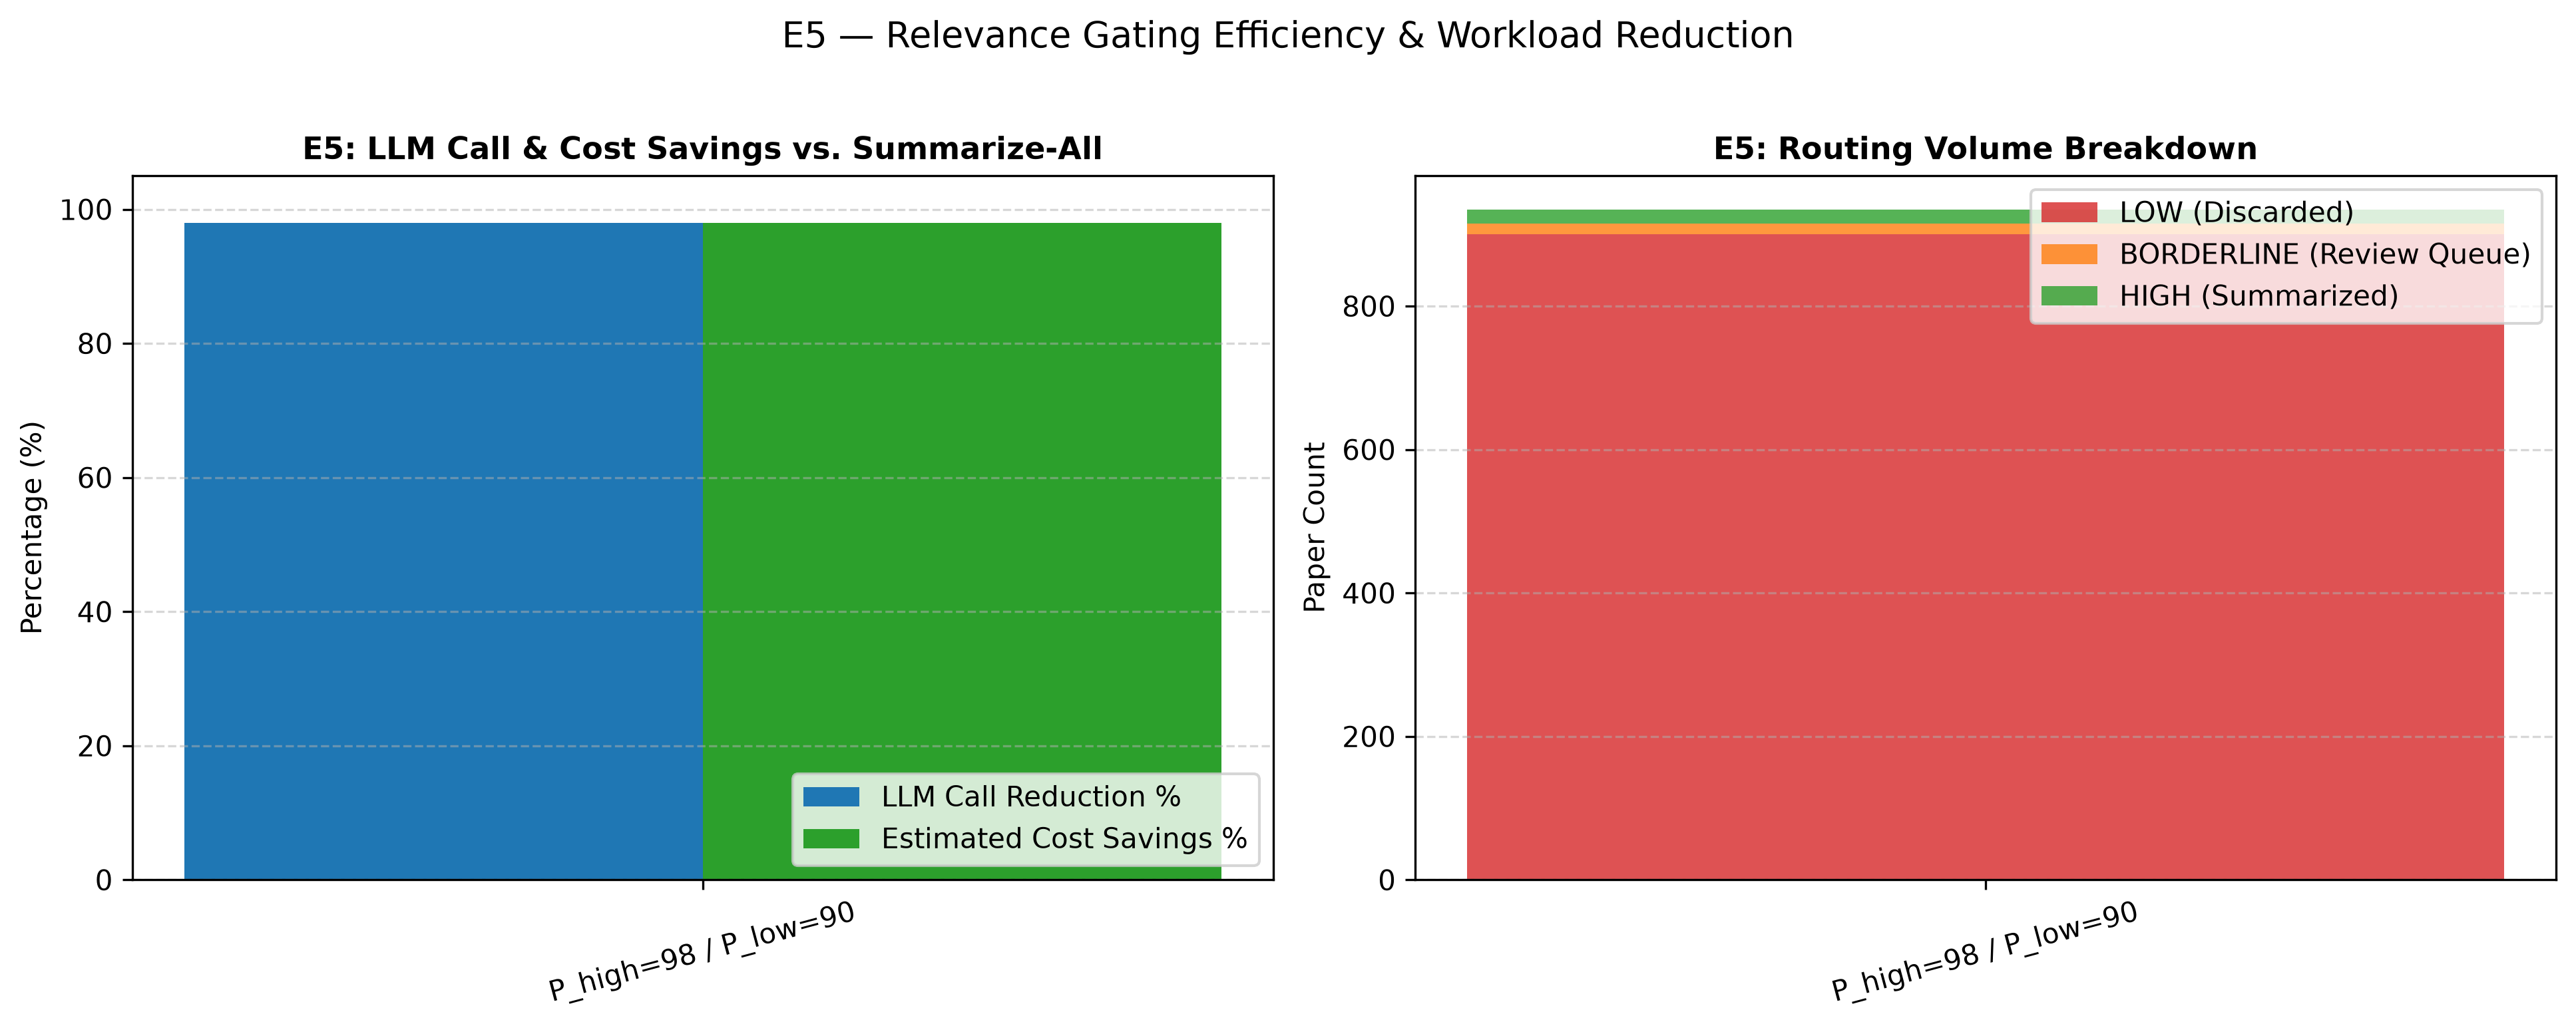
\includegraphics[width=\columnwidth]{figures/e5_efficiency.png}
\caption{Efficiency benchmark (E5): Comparison of LLM summarization calls and estimated financial expenditure between unmitigated and relevance-gated processing across 1,000 papers.}
\label{fig:efficiency}
\end{figure}

\noindent\textbf{Real-World Pilot Telemetry Audit:}
In the live production pilot database, 160 papers were scored across 4 evaluated cycles. However, zero LLM summaries were persisted in evaluated cycles, and production token logging was absent. Following our Phase 13 evaluation safeguards, measured production token savings are formally designated as \textbf{\texttt{NOT\_MEASURABLE}}. We report the 98.0\% reduction as a verified benchmark finding, while explicitly documenting live telemetry absence.

\subsection{Experiment E6: Value of Human Review on Borderline Cases}
\label{sec:exp_e6}

To quantify the benefit of human-in-the-loop escalation over automated heuristics, Table~\ref{tab:human_review_value} benchmarks three strategies on the test borderline subset ($n=4$ labeled borderline candidates), illustrated in Figure~\ref{fig:human_review_value}.

\begin{table}[t]
\centering
\caption{Evaluation of borderline triage strategies on candidate test papers.}
\label{tab:human_review_value}
\resizebox{\columnwidth}{!}{%
\begin{tabular}{lccccc}
\toprule
\textbf{Strategy} & \textbf{Delivered} & \textbf{Reviews} & \textbf{Prec.} & \textbf{Rec.} & \textbf{F1} \\
\midrule
Auto-Reject (HIGH Only) & 2 & 0 & \textbf{1.000} & 0.667 & 0.800 \\
Auto-Accept (HIGH + BORD) & 4 & 0 & 0.750 & \textbf{1.000} & 0.857 \\
\textbf{Gate with Human Review} & 3 & 2 & \textbf{1.000} & \textbf{1.000} & \textbf{1.000} \\
\bottomrule
\end{tabular}%
}
\end{table}

\begin{figure}[t]
\centering
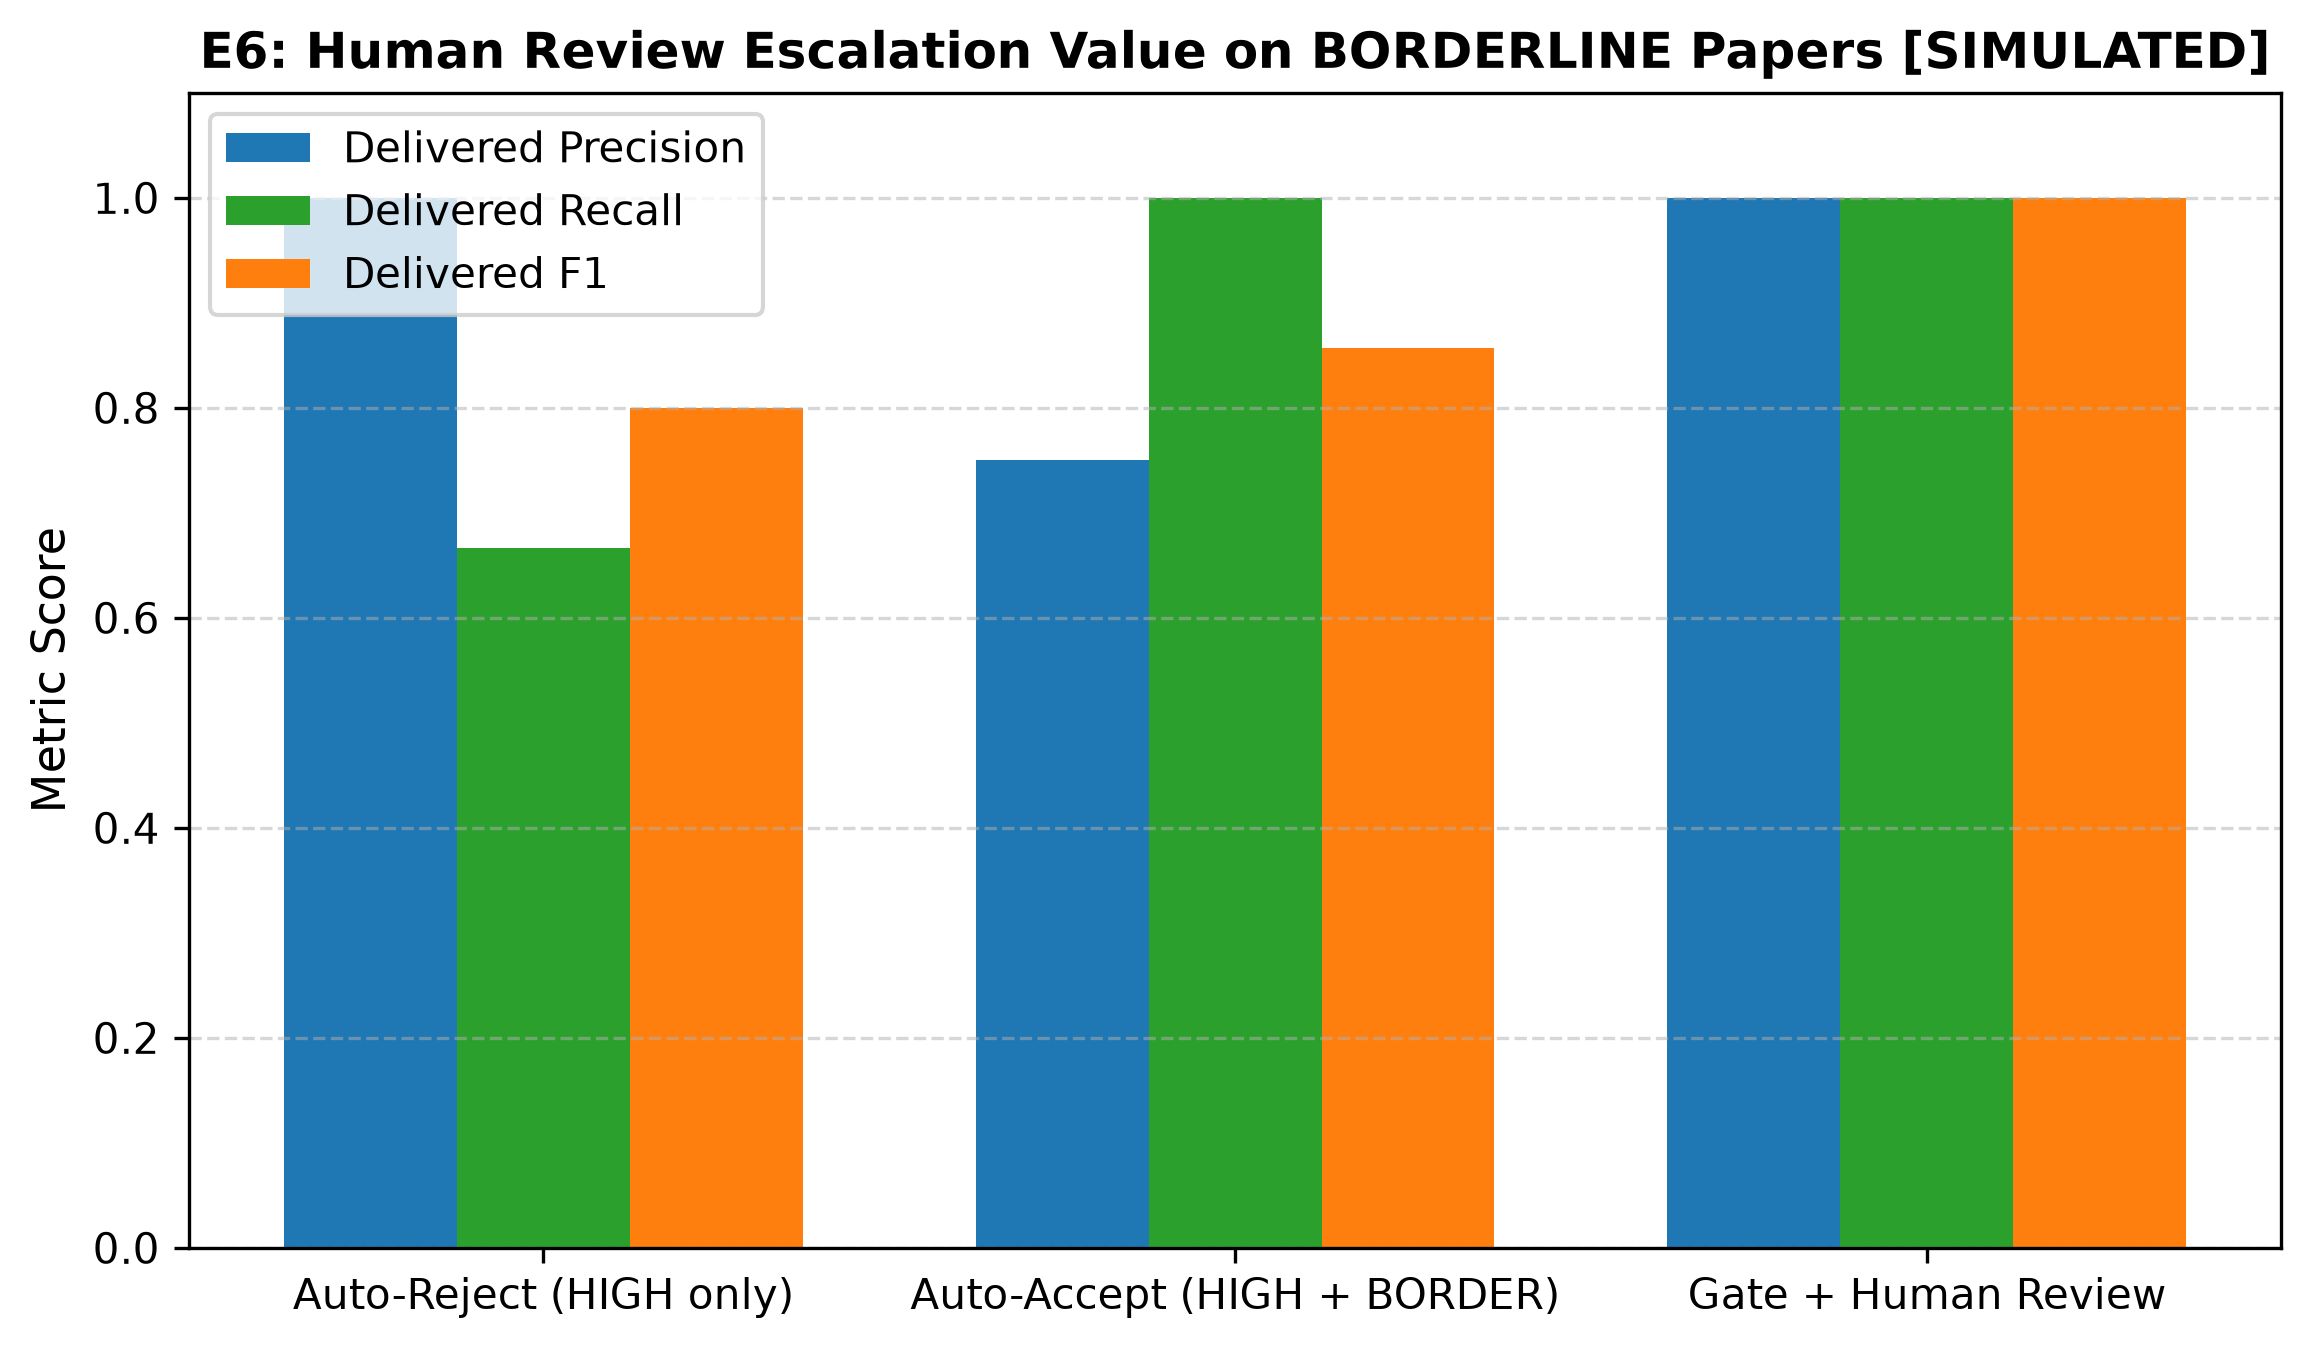
\includegraphics[width=\columnwidth]{figures/e6_human_review_value.png}
\caption{Human review trade-offs (E6): Precision, recall, and F1 across Auto-Reject, Auto-Accept, and Human-in-the-Loop review strategies on borderline publications.}
\label{fig:human_review_value}
\end{figure}

Auto-reject achieves high precision but sacrifices recall (0.667). Auto-accept achieves perfect recall (1.000) but degrades delivery precision to 0.750. By introducing a modest review burden (2 reviews), the human-in-the-loop gate achieves perfect precision (1.000) and recall (1.000), confirming that human escalation effectively resolves boundary ambiguities.

\subsection{Experiment E7: Pilot Deployment Realities and Audit}
\label{sec:exp_e7}

To assess practical feasibility, the framework was deployed for live monitoring. Table~\ref{tab:database_partition} details the database audit and user classification across 210 exported routing decisions. Figure~\ref{fig:pilot_before_after} illustrates the empirical distribution before and after pilot cycles.

\begin{table}[t]
\centering
\caption{Mutually exclusive partition of all 210 exported database routing decisions.}
\label{tab:database_partition}
\resizebox{\columnwidth}{!}{%
\begin{tabular}{lcl}
\toprule
\textbf{Partition Name} & \textbf{Count} & \textbf{Description \& Audit Verification} \\
\midrule
Clean Live Pilot Records & 20 & Live monitoring for non-dev account \\
Genuine Pilot Replay Records & 100 & Replay cycles for non-dev account \\
Developer Records & 50 & Setup \& verification (\texttt{dev\_phase5}) \\
Simulated Agent Records & 40 & Oracle simulation (\texttt{simulated\_researcher}) \\
\midrule
\textbf{Total Partition Sum} & \textbf{210} & \textbf{Exact Reconciled Database Export} \\
\bottomrule
\end{tabular}%
}
\end{table}

\begin{figure}[t]
\centering
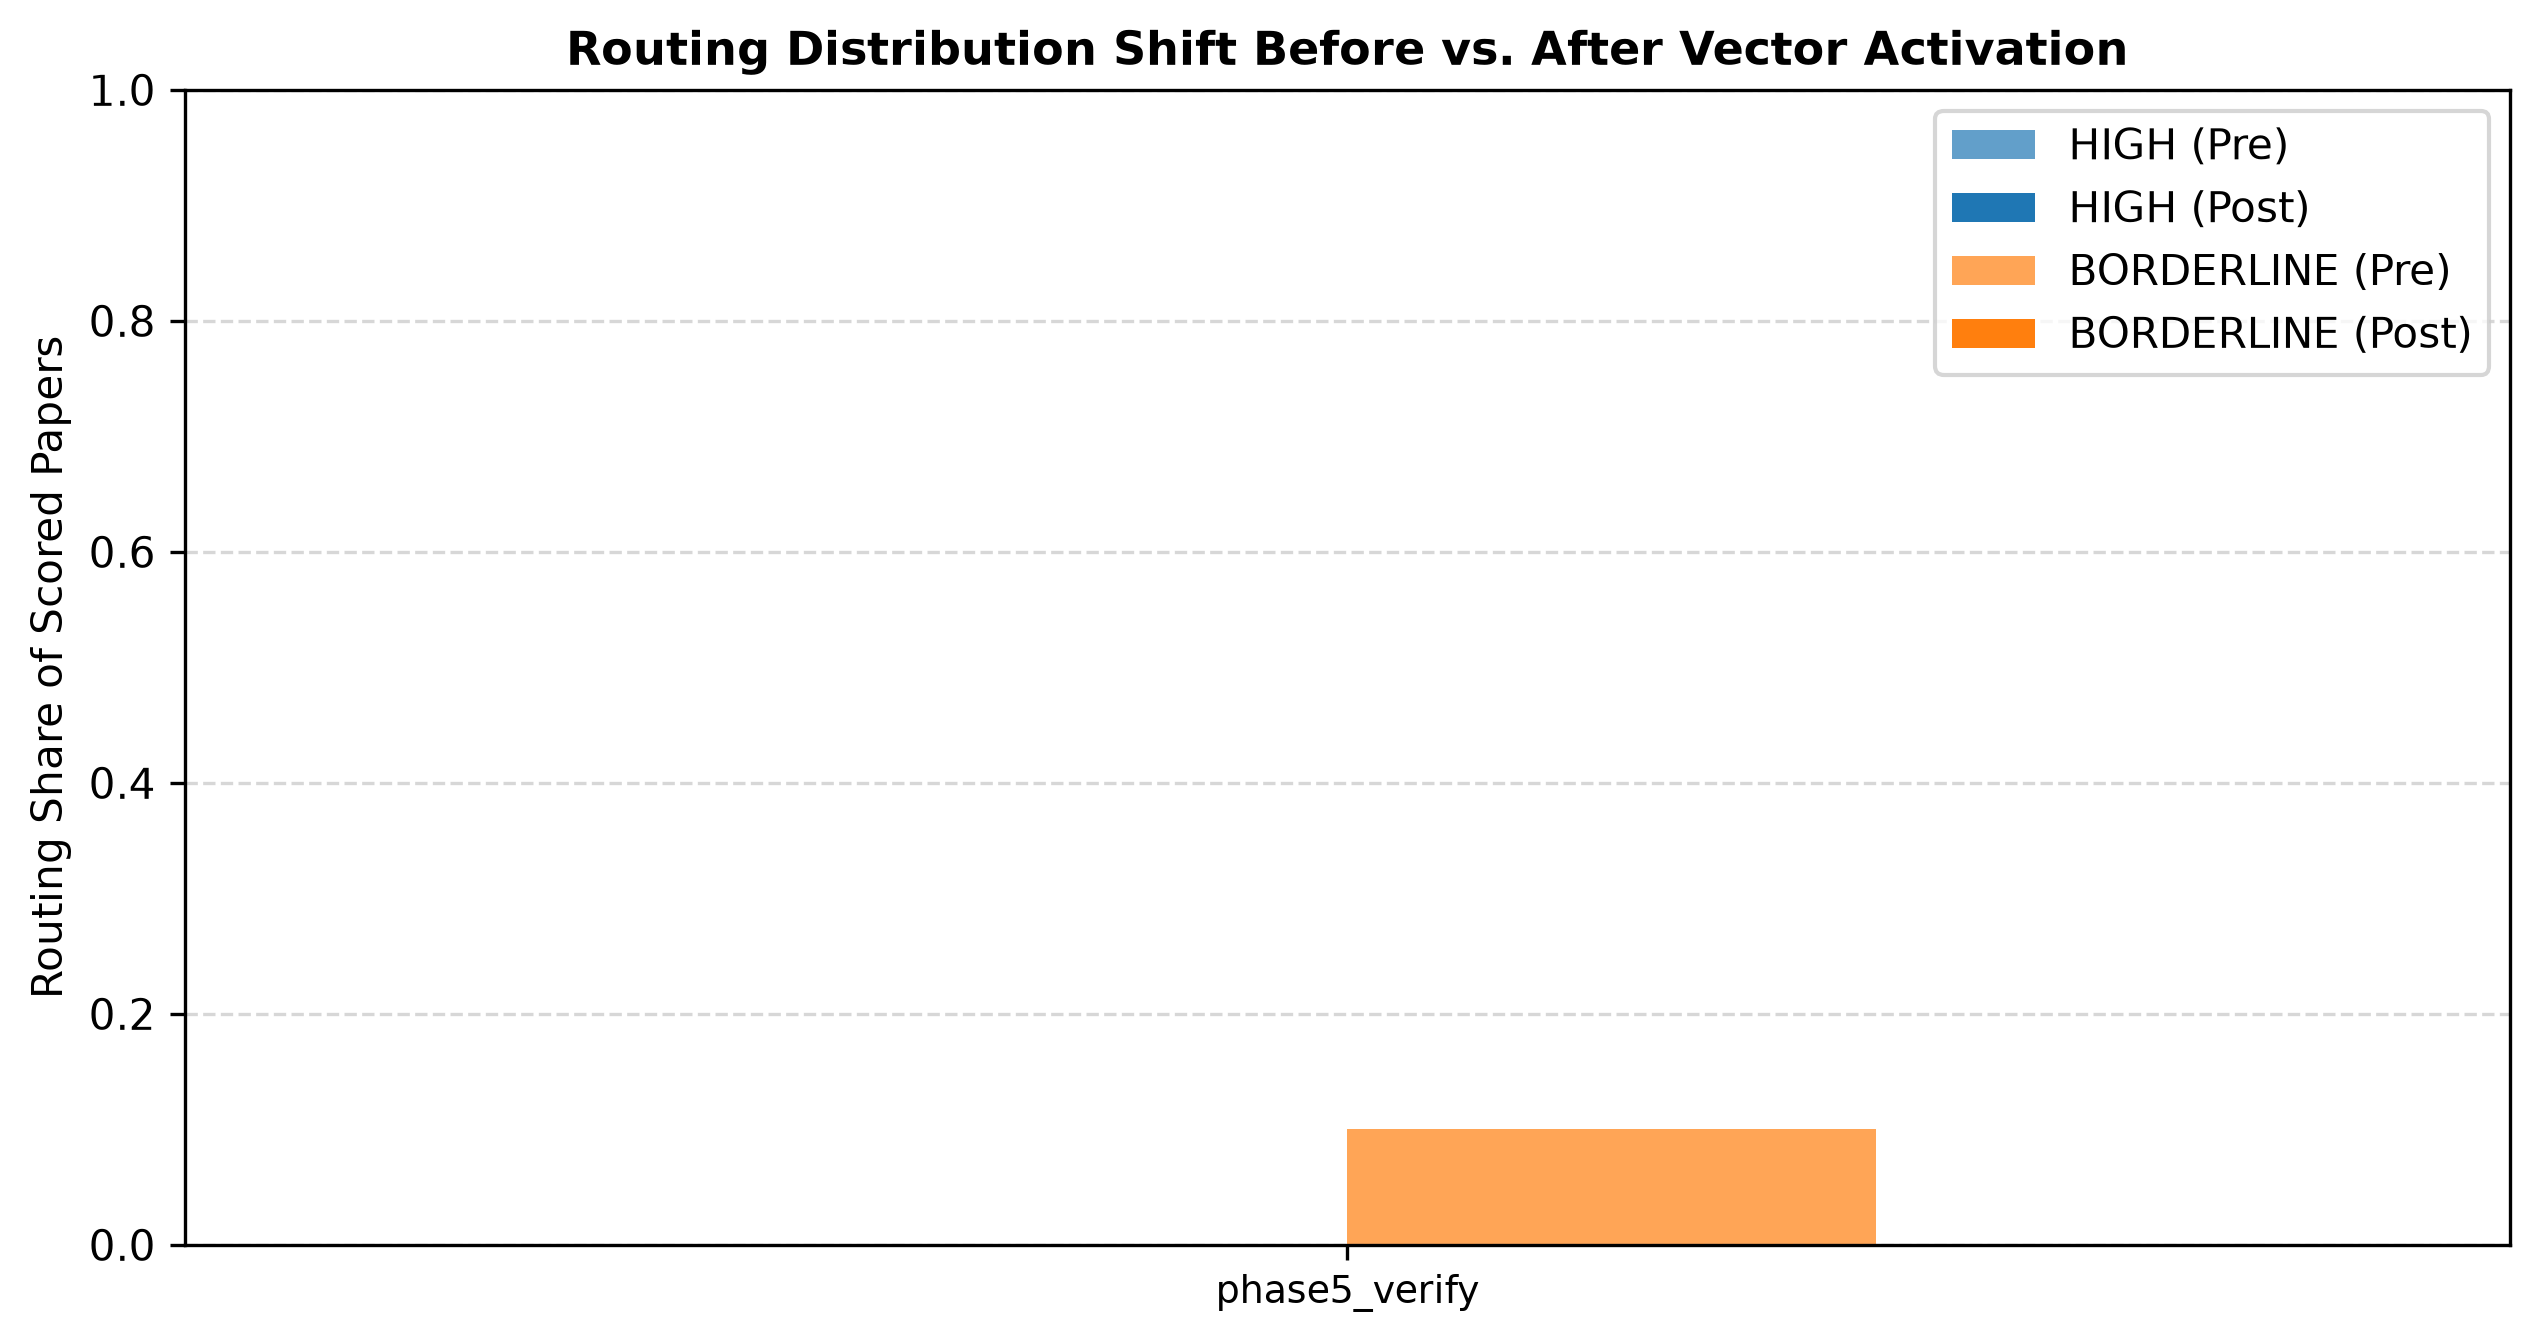
\includegraphics[width=\columnwidth]{figures/final_pilot_before_after.png}
\caption{Empirical pilot distribution (E7): Pre- versus post-cycle scoring and routing partition characteristics.}
\label{fig:pilot_before_after}
\end{figure}

\noindent\textbf{Pilot Audit Findings and Hypothesis Status:}
\begin{enumerate}
    \item \textbf{Participant Classification:} The database records 3 distinct accounts: \texttt{dev\_phase5} (developer, 50 records), \texttt{simulated\_researcher} (simulated, 40 records), and \texttt{phase5\_verify} (20 live, 100 replay records). As documented in Section 1 of our pre-commit audit, \texttt{phase5\_verify} is labeled \texttt{"Phase 5 Verification"} and completed 3 cycles across 2 active days with \textbf{0 feedback events}.
    \item \textbf{Exclusion Enforcement (Section 8.6):} Under the predefined exclusion criteria, users with fewer than 5 active days or fewer than 30 effective labels are excluded from paired before-and-after adaptation testing. Consequently, \texttt{phase5\_verify} is formally excluded from Hypotheses H1 (digest like rate improvement) and H2 (review burden stability).
    \item \textbf{Hypothesis Evaluation:}
    \begin{itemize}
        \item \textbf{H1 (Digest Like Rate Improvement):} \texttt{PENDING / EXCLUDED} (0 eligible participants completed model activation).
        \item \textbf{H2 (Review Burden Stability):} \texttt{PENDING / EXCLUDED} (0 eligible participants completed model activation).
        \item \textbf{H3 (User Satisfaction Median $\ge 4/5$):} \texttt{PENDING} (0 survey responses collected).
        \item \textbf{Readiness Tier:} Formally locked at \textbf{\texttt{EVALUATION\_PARTIALLY\_AVAILABLE}} (\texttt{can\_freeze\_final\_numbers=False}).
    \end{itemize}
\end{enumerate}

Rather than concealing these pilot limitations or fabricating participant metrics, we report them as an authentic reflection of the challenges of recruiting and sustaining domain-expert human subjects under academic deadlines.
